\chapter{Анализ основных причин джиттера в проводной и беспроводной сети} \label{chapt1}

\section{Конвергенция фиксированный и мобильных сетей} \label{sect1_1}
Эта раздел содержит обзор эволюции развития телекоммуникационных сетей в направлении конвергенции фиксированной и мобильной связи (FMC). Эта эволюция обусловлена снижением среднего дохода с потребителя услуг на мобильном и стационарном рынке потребления телекоммуникационных услуг, и конкуренция со стороны других технологий, а также из-за передачи голоса поверх IP сетей. FMC будет способствовать принятию сетей нового поколения \cite{FMC}, в которых весь коммуникационный трафик использует IP.
Существует несколько способов предоставления FMC услуг, некоторые из которых более технологически интегрированы, чем другие. Двух режимные телефоны сотовый/Wi-Fi которые используют Wi-Fi модемы в домашних условиях доступа к VoIP. Есть менее развитые формы FMC использующие двухрежимные телефоны сотовый/Wi-Fi, которые не имеют функции handover или имею эту функцию, но не используют ее для передачи голос или для доступа к широкополосной сети в домашних условиях. Также существуют услуги соединяющие мобильную и фиксированную сеть, которые технологически не происходит конвергенция, такие как предложение единого голосового и почтового ящика поверх фиксированный и мобильный сетей.
Концепция конвергенции фиксированной и мобильной широка, многогранна и развивается. Конвергенция происходит между устройствами, приложениями, сервис-контрольными механизмами и сетями. Конвергенция устройств происходит от camera phone до интеграции компьютера и телефона. Такие приложения, как электронная почта и управление взаимоотношениями с клиентами (CRM) становятся мобильными. На уровне управления услугами, в платформах управления политиками, идентификацией, и биллингом происходит конвергенция, создавая открытую систему, которая позволит предоставлять четыре вида услуг (данные, голос, видео и мобильность). Конвергенция сетей произошли в центре предоставления услуг, и в настоящее время также сходящихся в краю, где такие технологии, как Wi-Fi и wireless mesh становятся распространенными.
FMC продолжает развиваться по отдельности по каждому из этих параметров. Поставщики услуг представляют решения, которые отвечают потребностям своих абонентов. Эти решения, по сути, следуют традиционному жизненному циклу модели разработки программного обеспечения, который постепенно добавляет функциональности.
FMC услуги, подробное описание которых будет представлено в текущем разделе, представляет собой серьезную проблему для всех телекоммуникационных операторов в ближайшие несколько лет. Объединение разрозненных услуг по отдельным сетям стало рассматриваться как маркетинговый шаг, необходимый для поддержки заказчиков.
Несмотря на то, называемый «мобильный» сервис, сотовые беспроводные телефоны часто используются для не-телекоммуникационных функций и позволяет более точно учитывать персональные устройства связи. Они используются так часто в фиксированных местах, прежде всего, дома и в офисе, что некоторые операторы предлагают специальные «домашней зоне» тарифов, а в других мобильных конкурирует непосредственно с ограниченным диапазоном основных беспроводного доступа (FWA).
В то время как клиенты все чаще используют сеть радиодоступа (RAN) на короткие расстояния, большая часть транспортной трафика осуществляется на основных сетей, построенных с оптических кабелей. Они предлагают высокую производительность и низкую себестоимость, что нынешняя много преимуществ. Во многих малых островных развивающихся государств (МОРГ) использование спутниковых неизбежно, потому что нет никаких подводных кабелей, что значительно увеличивает расходы. В большинстве стран Африки существует ограниченное предоставление подводного кабеля или доступ к ним кабелей контролируется монополией.
Сила продолжает инновации необходимы усилия наметить закономерности технологического развития, например, в эволюции сетей широкополосного доступа и услуг. Эти попытки прогнозирования указывают на будущее, что будет продолжать меняться. Карты должны быть изменены, как только они вступают в контакт с потребителями, чьи ответы оказались настолько непредсказуемы.
С учетом задержек и неопределенностей во введении третьего поколения (3G), услуги мобильной связи, производители разработали планы Long Term Evolution (LTE) в 3.5G и за ее пределами. Они предназначены для того, чтобы избежать перерыва в течение введение 4G и потенциально крайне непопулярны требования для финансирования крупных инвестиций в новую инфраструктуру. Тем не менее, избежать термин 4G она остается открытой для использования поставщиками альтернативных технологий, стремясь получить маркетинговые преимущества по сравнению с 3G операторами. На фиксированных сетей, терминология является расплывчатой Next Generation Network (NGN) используется, хотя некоторые из технологий является общим.

\section{Обзор концепции потоковых агентов} \label{sect1_2}
При передаче мультимедийной информации по комбинированным сетям с учетом различных механизмов распространения с различными технологиями, важным является выполнение требований по качеству предоставления мультимедийной информации пользователю.
При этом важными являются такие характеристики: задержка, число потерянных и поврежденных пакетов. Как показывает практика наибольшие потери качественных характеристик происходит на границах операторских сетей и сетей с различными механизмами распространения.
Возникает необходимость установки соответствующих агентов, обеспечивающих мониторинг на том или ином промежутке сети. Вместе с тем от числа и места этих агентов существенно зависит качество мониторинга.
Потоковый агент (ПА) это агент, который находится на базовой станции на пересечении проводной и беспроводной сети (рис. \ref{img:SA}). Агент просматривает и распознает поток, исследуя заголовки RTP. Агент периодически посылает статистические и своевременные обратные сообщения на отправляющий сервер. Статистические обратные связи помогают отправителю проследить проводное состояние сети, что существенно для выполнения надлежащего контроля над перегрузками. С другой стороны, потоковый агент отправляет своевременные обратные сообщения, такие как подтверждение пакетов (ACKs), что говорит отправителю о прибытии каждого пакета к агенту корректно и вовремя.


\begin{figure} [h]
  \center
\includegraphics [width=0.95\textwidth] {SA.eps}
  \caption{Использование ПА}
  \label{img:SA}
\end{figure}

Блок формирования находится перед ПА и ограничивает объем отправляемых сообщений, чтобы он не был больше чем полоса пропускания беспроводной сети, храня пакеты, ожидающие фрагментации и передачи на более низкий уровень. Если состояние беспроводной сети плохое число повторных передач будет расти, заставляя увеличиваться очередь пакетов. Блок формирования реагирует на заполненность очереди, отбрасывая пакеты до прибытия их к агенту.

ПА позволяет выполнять множество функций для улучшения качества предоставления мультимедийных услуг:
\begin{itemize}
\item ПА предоставляет дополнительную обратную связь для контент сервера с границы между проводной  и беспроводной частью сети \cite{SAdouble_feedback}.
\item ПА дает возможность определить место пакетной ошибки \cite{SAdouble_feedback}, что позваляет корректно реагировать на потери и задержки в сети.
\item Ретрансляция на прикладном уровне позволяет уменьшить  пакетные искажения  для приложений не восприимчивых к задержке \cite{SArateOpt, SArealtime}.
\item Прямая коррекция ошибок позволяет уменьшить битовые искажения для приложений восприимчивых к задержке \cite{SArateOpt, SArealtime}.
\end{itemize}






\section{Анализ архитектуры беспроводной сети LTE} \label{sect1_3}
Сеть LTE состоит из двух важнейших компонентов \cite{lte}: сети радиодоступа E-UTRAN, базовой сети SAE (System Architecture Evolution) (рис. \ref{img:LTEscheme}).
\begin{figure} [h]
  \center
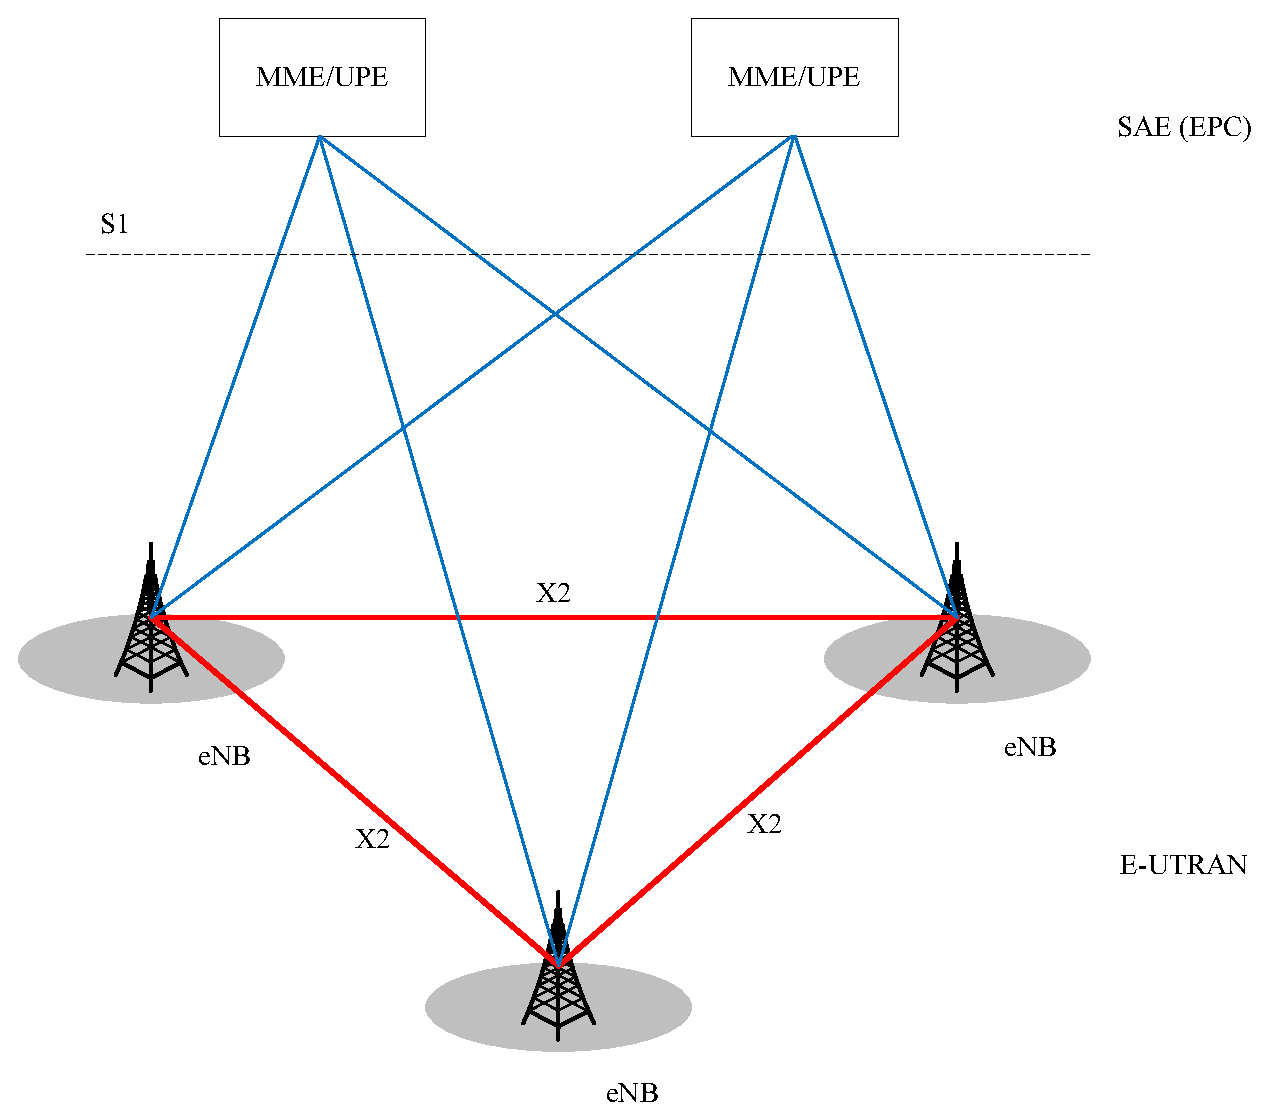
\includegraphics [width=0.8\textwidth] {LTEscheme.eps}
  \caption{Взаимодействие сети радиодоступа E-UTRAN и базовой сети SAE}
  \label{img:LTEscheme}
\end{figure}

Основными требованиями проекта 3GPP к сети SAE были: максимально возможное упрощение структуры сети и исключение дублирующих функций сетевых протоколов, характерных для систем UMTS.
Сети радиодоступа E-UTRAN рассмотрена в ряде технических спецификаций, согласно которым она состоит только из базовых станций eNB (evolved Node B). Базовые станции eNB являются элементами полносвязной сети E-UTRAN и соединены между собой по принципу каждый с каждым при помощи интерфейса X2. Интерфейс X2 поддерживает хендовер мобильного терминала в состоянии LTE\_ACTIVE. Каждая базовая станция имеет интерфейс S1 с базовой сетью SAE, построенный по принципу коммутации пакетов.
Базовая сеть SAE \cite{lte}, иногда называемая сетью EPC (Evolved Packet Core), содержит узлы MME/UPE, состоящие из логических элементов MME и UPE. Логический элемент MME (Mobility Management Entity) отвечает за решение задач управления мобильностью абонентского терминала и взаимодействует с базовыми станциями eNB сети E-UTRAN с помощью протоколов плоскости управления C-plane (интерфейс S1-C). Логический элемент UPE (User Plane Entity) отвечает за передачу данных пользователей согласно протоколам плоскости пользователя U-Plane и взаимодействует с eNB посредством интерфейса S1-U.
Благодаря интерфейсу S1 базовые станции соединены с несколькими узлами MME/UPE, что позволяет более гибко использовать сетевой ресурс. Такой интерфейс называют S1-flex.
Сеть LTE имеет следующие функциональные отличия от сети UMTS.

\begin{enumerate}
  \item Базовые станции eNB выполняют функции управления радиоресурсами RRM (Radio Resource Management): управление радиоканалами (Radio Bearer Control), управление доступом (Radio Admission Control), управление мобильностью (Connection Mobility Control), динамическое распределение ресурсов (Dynamic Resource Allocation). Таким образом, в сети радиодоступа E-UTRAN базовые станции eNB управляют протоколами радиоинтерфейса, комбинируя выполнение функций базовых станций Node В и большинство функций контроллера RNC сети UMTS.
  \item Сетевой элемент управления мобильностью MME отвечает за распределение сообщений вызова (paging) к базовым станциям eNB. Кроме того, MME управляет протоколами плоскости управления: назначения идентификаторов абонентских терминалов, обеспечения безопасности сети, проверки подлинности сообщений абонентов и управления роумингом.
  \item Сетевой элемент плоскости пользователя UPE выполняет сжатие заголовков IP-протоколов, шифрование потоков данных, терминацию пакетов данных плоскости пользователя, коммутацию пакетов данных при обеспечении мобильности пользователя. Кроме того, UPE управляет протоколами пользовательского уровня, например, хранением текущего статуса абонентского терминала (АТ), прерыванием состояния LET\_IDLE на уровне абонентских терминалов.
\end{enumerate}
Основные протоколы интерфейса S1 плоскостей C-plane и U-plane сети LTЕ представлены на рис. \ref{img:LTEinterface}.
\begin{figure} [h]
  \center
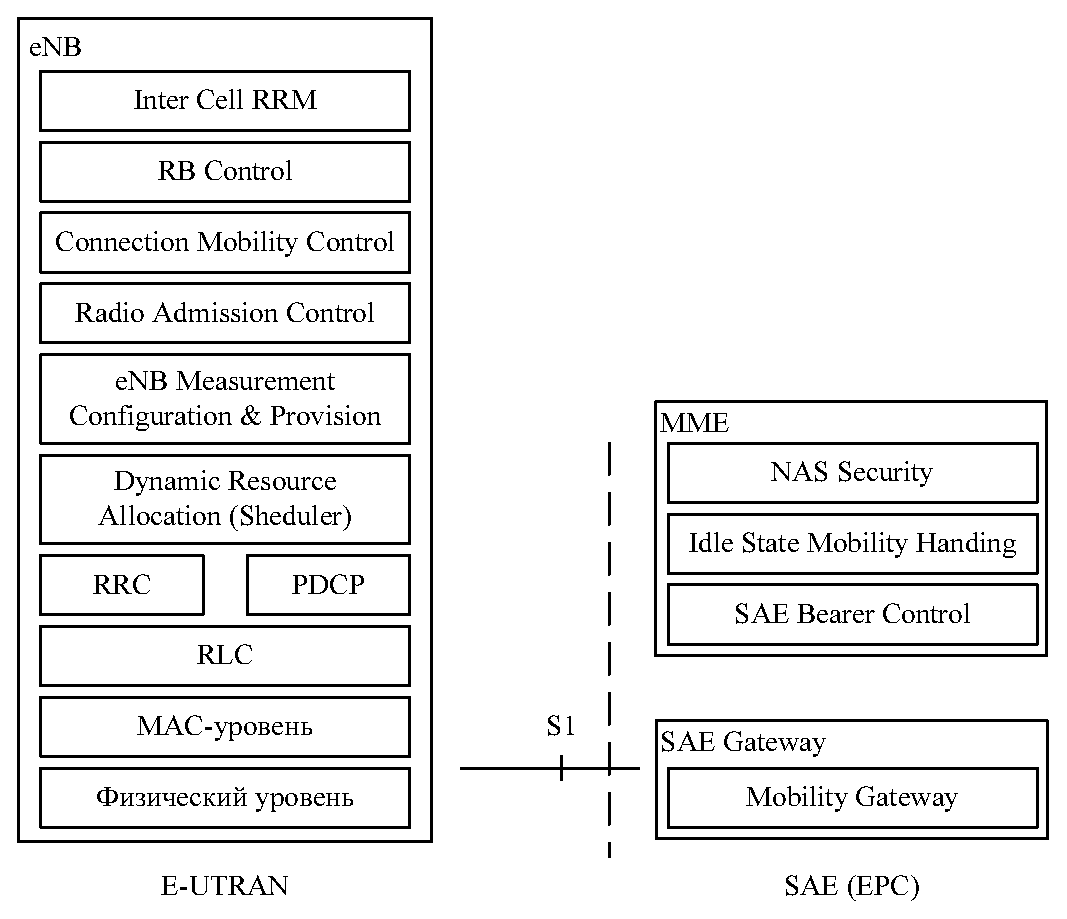
\includegraphics [width=0.6\textwidth] {LTEinterface.eps}
  \caption{Протоколы интерфейса S1 сети LTE}
  \label{img:LTEinterface}
\end{figure}
Одной из важнейших задач управления в сети LTE является максимально эффективное использование радиоресурсов. Данная задача решается с помощью совокупности функций управления радиоресурсами RRM (управление радиоресурсами сети E-UTRAN, управление службой передачи данных в радиоканале, управление мобильностью, управление доступом, динамическое распределение ресурсов) и с помощью протокола управления радиоресурсами RRC. 
Управление радиоресурсами сети E-UTRAN (Inter Cell RRM) обеспечивает управление ресурсами группы сот в целях повышения эффективности использования частотного спектра и минимизации помехового взаимного влияния абонентских терминалов и базовых станций, а также поддержку мобильности.
Управление службой передачи данных в радиоканале (RB Control) реализовано в базовых станциях eNB сети E-UTRAN и обеспечивает установление, поддержание и освобождение радиоканалов передачи данных с заданными параметрами в сети E-UTRAN. Основными задачами являются контроль и управление всеми активными сессиями передачи данных с учетом параметров качества услуг (QoS), выделение ресурсов для вновь активируемых сессий.
Управление мобильностью (Connection Mobility Control) позволяет выбирать обслуживающую базовую станцию eNB для мобильного терминала, передавать обслуживание мобильного терминала от одной базовой станции eNB (хэндовер) к другой. Выбор обслуживающей eNB осуществляется мобильным терминалом на основе собственных измерений в состоянии RRC\_CONNECTED и сравнения полученных измерений с установленными пороговыми значениями. Хэндовер реализован на основе анализа измерений как мобильного терминала, так и базовой станции eNB, а также текущей загрузки обслуживающей и соседних сот, политикой оператора по регулированию трафика.
Поддержку мобильности абонентского терминала в сети SAE обеспечивает логический элемент MME. Основными функциями MME являются:
\begin{itemize}
  \item Управление мобильностью абонентского терминала, находящегося в состоянии RRC\_IDLE (Idle State Mobility Handling).
  \item Управление безопасностью мобильной связи (NAS Security) в соответствии с протоколами, относящимися к группе протоколов «уровня без доступа» и обеспечивающими, например, аутентификацию пользователей, управление ключами шифрования данных.
  \item Управление службой передачи данных сети SAE (SAE Bearer Control).
\end{itemize}
Параметры функций управления радиоресурсами сети E-UTRAN (Inter
Cell RRM), управления службой передачи данных в радиоканале (RB Control) и управления мобильностью (Connection Mobility Control) могут быть кастомизированы в соответствии с требованиями оператора.
Основной задачей управления доступом (Radio Admission Control) является формирование решений о предоставлении доступа мобильному терминалу к сети E-UTRAN. Данная задача решается на основе многокритериального анализа загрузки сети радиодоступа, требований мобильного терминала к параметрам QoS.
Динамическое распределение ресурсов (Dynamic Resource Allocation; Scheduler) отвечает за планирование очередности передачи пакетов данных и позволяет динамически выделять и перераспределять ресурсы сети радиодоступа, включая канальные ресурсы, мощность излучения базовых станций, ресурсы буферизации при обработке пакетов данных с учетом параметров QoS.
Протокол управления радиоресурсами RRC плоскости С-plane обеспечивает:
\begin{itemize}
  \item Вещание служебной информации в соответствии с протоколами, относящимися к группам протоколов «уровня с доступом» и «уровня без доступа» (соответственно AS - Access Stratum и NAS - Non-Access Stratum).
  \item Пейджинг мобильного терминала.
  \item Установление, поддержание и закрытие RRC-соединений между абонентским терминалом и сетью E-UTRAN.
  \item Управление ключами шифрования.
  \item Установление, поддержание и закрытие служб передачи данных в радиоканале (Radio Bearers) типа «точка-точка» и «точка-многоточка» с заданными параметрами QoS.
  \item Мобильность абонентских терминалов.
\end{itemize}
Кроме того, протокол RRC обеспечивает выполнение ряда других функций.
Протокол сходимости пакетных данных PDCP (Packet Data Convergence Protocol) плоскостей U-plane и C-plane обеспечивает устранение избыточности (сжатие) служебной информации, объем которой может быть соизмерим с объемом полезной информации, передаваемой в пакетах данных, а также шифрование/дешифрование данных.
Протокол управления радиоканалом RLC (Radio Link Control) обеспечивает:
\begin{itemize}
  \item Сегментацию и компоновку пакетов данных протоколов более высокого уровня PDU (Protocol Data Unit) переменной длины в меньшие блоки полезной нагрузки PU (Packet Unit); размер блока PU определяется в соответствии со скоростью передачи информации в радиоканале.
  \item Конкатенцию (сочленение) коротких пакетов PDU верхнего уровня.
  \item Заполнение остатка поля данных блока PU, если сочленение неприемлемо.
  \item Передачу данных пользователя с подтверждением и неподтверждением приема в соответствии с параметрами QoS.
  \item Исправление ошибок методом повторной передачи (ARQ) пакетов данных.
  \item Сохранение на более высоком уровне порядка доставки пакетов PDU при передаче данных с подтверждением приема.
  \item Обнаружение дублирования пакетов PDU для доставки их на более высокий уровень только один раз.
  \item Управление скоростью передачи данных.
  \item Контроль порядковых номеров пакетов.
\end{itemize}
Архитектура базовой сети SAE позволяет осуществлять дальнейшую эволюцию сетей 3G в направлении получения более высоких скоростей передачи данных, обеспечения низких задержек, а также оптимизации передачи данных на основе разнообразных технологий радиодоступа. Основным от личием базовой сети SAE от базовой сети системы UMTS является максимально упрощенная структура и отсутствие дублирующих функций сетевых протоколов.
Архитектура базовой сети SAE представляет собой PS-домен системы LTE, который предоставляет как голосовые услуги, так и всю совокупность IP-услуг на основе технологий пакетной коммутации данных. В основу построения базовой сети SAE положена концепция «все через IP» (all-IP или AIPN — All over IP Network) и то обстоятельство, что доступ к базовой сети SAE может осуществляться как через сети радиодоступа второго и третьего поколений (например, сети UTRAN, GERAN), так и через сети радиодоступа неевропейских технологий, не стандартизированные проектом 3GPP (сети He-3GPP), например, сети IEEE: Wi-Fi, WiMAX, а также через сети, использующие проводные IP-технологии (например, сети ADSL+, FTTH и др.).
Эталонная архитектура базовой сети SAE с указанием интерфейсов взаимодействия с внешними сетями показана на рис. \ref{img:SAEnetwork}. Согласно этой архитектуре функции протоколов плоскости управления узла SGSN сети UMTS становятся функциями элемента управления мобильностью MME. Функции контроллера RNC, которые не выполняет базовая станция eNB сети E-UTRAN, и функции протоколов плоскости пользователя узлов SGSN и GGSN реализуются модулем UPE и шлюзовым узлом «привязки» 3GPP Anchor сети SAE. Этот узел предназначен для присоединения сетей 2G/3G к сети LTE. В состав SAE входит также шлюзовый узел привязки SAE Anchor, который служит для присоединения к сети SAE сетей стандартов 3GPP (GSM/UMTS) и стандартов нe-3GPP (Wi-Fi и WiMAX). Узлы привязки 3GPP Anchor и SAE Anchor образуют единый узел привязки IASA (Inter Access System Anchor) для присоединения внешних IP-сетей.
Совокупность логических сетевых элементов MME/UPE, IASA, состоящего из узлов SAE Anchor и 3GPP Anchor (рис. \ref{img:SAEnetwork}), образует базовую пакетную сеть (Evolved Packet Core — ЕРС). Данные логические элементы рассматривались в основном на начальных стадиях разработки стандартов сети LTE. Более детальные исследования, направленные на практическую реализацию архитектуры ЕРС, определили новые сетевые элементы: обслуживающий шлюз S-GW (Serving GW) и шлюз взаимодействия с пакетными сетями P-GW (PDN GW), а также логический элемент MME, функционирующий отдельно от элемента UPE. Шлюзы S-GW и Р-GW физически могут быть реализованы в составе одного сетевого элемента AGW (Access GW).
Краткое описание основных интерфейсов сети SAE приведено в табл. \ref{SAEinterface}.
\begin{figure} [h]
  \center
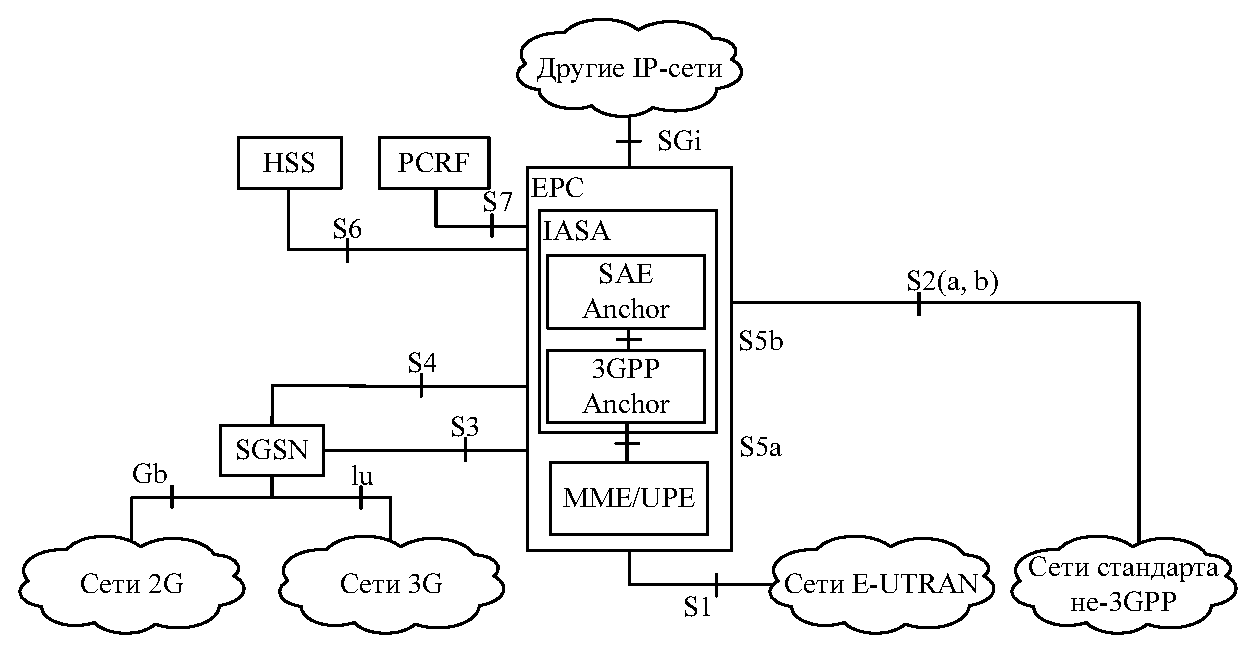
\includegraphics [width=0.95\textwidth] {SAEnetwork.eps}
  \caption{Эталонная архитектура базовой сети SAE}
  \label{img:SAEnetwork}
\end{figure}

\begin{table} [htbp]
  \centering
  \parbox{15cm}{\caption{Основные интерфейсы сети SAE}\label{SAEinterface}}
%  \begin{center}
  \begin{tabular}[t]{| p{3cm} || p{12cm}l |}
  \hline
  \hline
  Интерфейс & \centering  Описание интерфейса & \\
  \hline
  \hline
  S1 & \centering  Интерфейс, предоставляющий доступ к сети радиодоступа E-UTRAN для передачи данных протоколов плоскостей пользователя и управления. Позволяет иметь раздельную и комбинированную аппаратную реализацию элементов MME и UPE & \\
  \hline
  S2a & \centering Интерфейс между узлом IASA и фиксированными IP-сетями стандарта нe-3GPP. Обеспечивает передачу данных протоколов плоскости пользователя и поддержку функций управления и мобильности. Включает в себя интерфейсы S2a, S2b и S2c & \\
  \hline
  S3 & \centering Интерфейс между элементами MME/UPE и узлом SGSN. Обеспечивает управление межсетевым хэндовером абонентских терминалов в сетях E-UTRAN и UTRAN  & \\
  \hline
  S4 & \centering Интерфейс между узлом 3GPP Anchor и узлом SGSN. Обеспечивает передачу данных плоскости пользователя и поддержку функций управления и мобильности. Основан на интерфейсе Gn между узлами SGSN и GGSN сети UMTS  & \\
  \hline
  S5a & \centering Интерфейс между элементом MME/UPE и узлом 3GPP Anchor. Обеспечивает передачу данных протоколов плоскости пользователя и поддержку функций управления и мобильности  & \\
  \hline
  S5b & \centering Интерфейс между узлами 3GPP Anchor и SAE Anchor. Обеспечивает передачу данных протоколов плоскости пользователя и поддержку функций управления и мобильности   & \\
  \hline
  S6 & \centering Интерфейс, обеспечивающий доступ к домашней базе данных пользователей (HSS) для аутентификации и авторизации пользователей (интерфейс ААА) & \\
  \hline
  S7 & \centering Интерфейс, обеспечивающий управление установлением соединений с заданными параметрами QoS на основе политики сети и тарификацию (Policy and Charging Rules Function — PCRF)    & \\
  \hline
  SGi & \centering Интерфейс между узлом IASA и внешними сетями с пакетной передачей данных. Эти сети могут принадлежать как разным операторам, так и одному оператору сотовой связи для предоставления, например, услуг подсистемы IMS. Этот интерфейс основан на интерфейсе Gi между узлами GGSN и внешними IP-сетями  & \\
  \hline
  \hline
  \end{tabular}
%  \end{center}
\end{table}




======================================================================

(в процессе!!!!!!!!!!!!!!!!)

======================================================================

Для того чтобы рассчитать влияние SINR на скорость в канала рассмотрим формирование кадров в LTE (рис. \ref{img:frame_lte}). Рассмотрим нисходящее направление соединения и предположим что соединение между UE и eNB уже было установленно. Данные сначала поступают на PDCP (Packet data compression protocol) уровень. Этот уровень выполняет сжатие и шифрование данных и если необходимо устанавливает проверку на целосность. Далее данные передаются на RLC (LTE Radio Link Control) уровень, который объединяет PDCP PDUs в один RLC PDU.

RLC уровень объединит или сегментирует данные, поступающие от уровня PDCP в правильный размер блока и направит его на уровень МАС со своим собственным заголовком. Теперь MAC уровень выбирает схему модуляции и кодирования настраиваемую на физическом уровне. Теперь эти данные включенные в транспортный блок, должны быть переданы в 1 мс подкадре.

Теперь, сколько битов передаются в этом 1 мс размер транспортного блока? Это зависит от MCS (схемы модуляции и кодирования) и количество ресурсных блоков назначены UE. Мы должны обратиться к таблице 7.1.7.1-1 и таблице 7.1.7.2.1-1 от \cite{3GPPTS36213}.

%\clearpage
\begin{figure} [h]
  \center
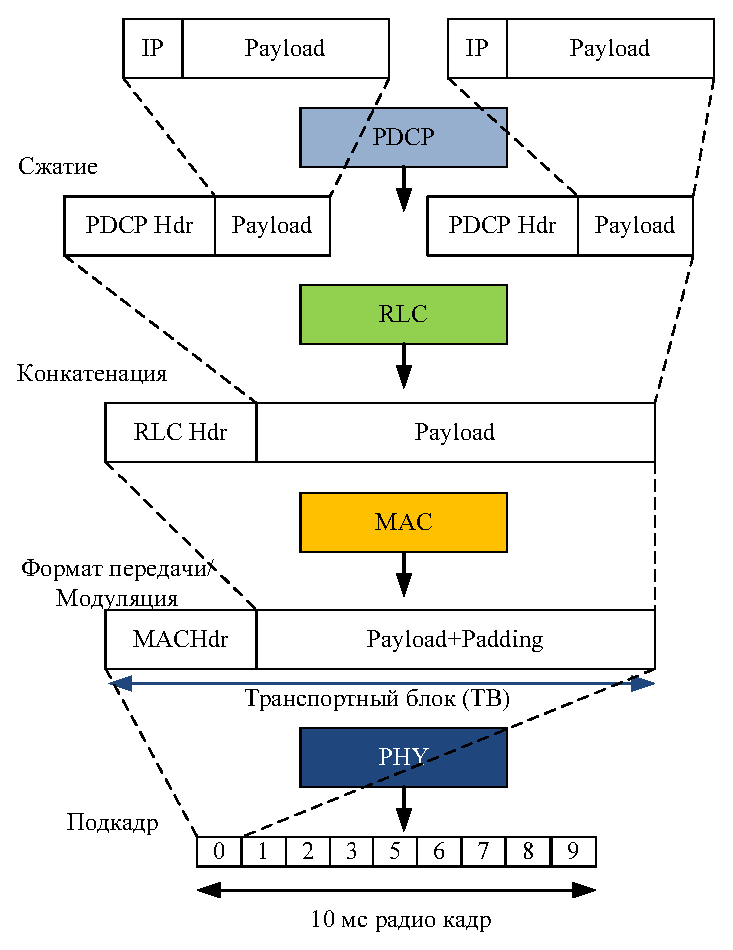
\includegraphics{frame_lte.eps}
  \caption{Формироваие транспортного блока (TB) в LTE}
  \label{img:frame_lte}
\end{figure}










\section{Архитектура имитационной модели LTE в NS3} \label{sect1_4}
Обзор имитационной модели LTE-EPC изображен на рис. \ref{img:LTEEPC}. Состоит из двух основных компонентов:
\begin{itemize}
  \item Модель LTE. Эта модель включает LTE радио стек протоколов (RRC, PDCP, RLC, MAC, PHY). Эти объекты полностью находятся на UE и eNB узлах.
  \item Модель EPC. Эта модель включает в себя основные сетевые интерфейсы, протоколы и объекты. Эти объекты и протоколы находятся на S-GW, P-GW и MME узлах и частично на eNB узлах. 
\end{itemize}

\begin{figure} [h]
  \center
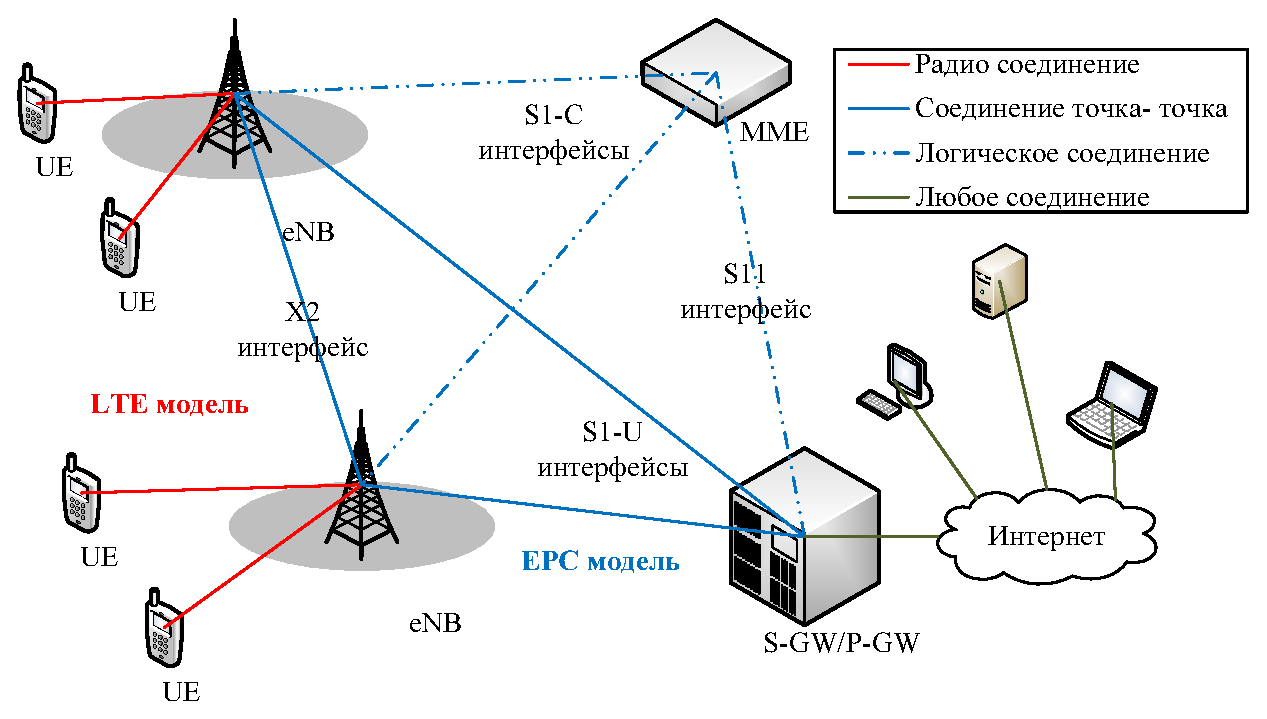
\includegraphics [width=0.95\textwidth] {LTEEPC.eps}
  \caption{Обзор имитационной модели LTE-EPC \cite{LteSimDoc}}
  \label{img:LTEEPC}
\end{figure}



\subsection{Архитектура LTE модели} \label{sect1_4_1}
LTE модель была разработана для поддержки оценки следующих аспектов системы LTE:
\begin{itemize}
  \item Управление радио ресурсами.
  \item Пакетная обработка на основе QoS.
  \item Внутрисистемные помехи между сотами.
  \item Динамический спектральный доступ
\end{itemize}


Архитектура физического и канального уровня для модели узла UE представлена на рис. \ref{img:UEPHY} и для модели узла eNB представлена на рис \ref{img:eNBPHY}.
\begin{figure} [h]
  \center
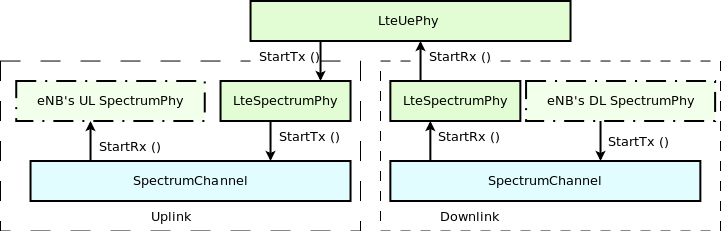
\includegraphics [width=0.95\textwidth] {UEPHY.png}
  \caption{Архитектура физического и канального уровня для модели UE \cite{LteSimDoc}}
  \label{img:UEPHY}
\end{figure}

\begin{figure} [h]
  \center
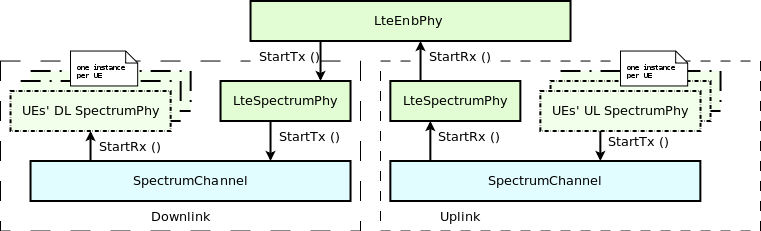
\includegraphics [width=0.95\textwidth] {eNBPHY.png}
  \caption{Архитектура физического и канального уровня для модели eNB \cite{LteSimDoc}}
  \label{img:eNBPHY}
\end{figure}


\subsection{Архитектура EPC модели} \label{sect1_4_2}
Модели EPC обеспечивает средства для моделирования сквозного IP соединения по верх LTE модели. В частности, поддерживает соединение нескольких UE с интернетом через сеть радиодоступа с несколькими узлами eNB, подключенными к одному SGW/PGW узлу. Эта топология сети изображен на рис \ref{img:LTEEPCdata}.
Основное внимание в модели ЕРС в настоящее время сфокусировано на плоскости данных EPC. Чтобы понять архитектуру этой модели, мы сначала посмотрим на рис \ref{img:LTEEPCdata}, где представлен сквозной LTE-EPC стек протоколов таким образом каким это реализовано в симуляторе. Из рисунка видно, что самые большие упрощения введены в модели ЕРС для плоскости данных, является включение функций SGW и PGW в один узел SGW / PGW, который устраняет необходимость S5 или S8 интерфейсов, определенных в 3GPP . С другой стороны, все уровни протокола S1-U и протокола радиосвязи LTE стек, указанные в 3GPP, присутствуют.

\begin{figure} [h]
  \center
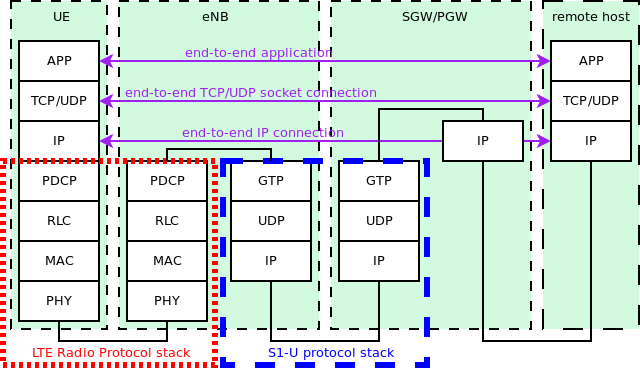
\includegraphics [width=0.95\textwidth] {LTEEPCdata.png}
  \caption{Архитектура физического и канального уровня для модели eNB \cite{LteSimDoc}}
  \label{img:LTEEPCdata}
\end{figure}

Как показано на рисунке, существует два различный уровня IP-сети. Первый это сквозной уровень, который обеспечивает сквозное подключение к пользователям; этот слой включает UE, PGW и удаленный хост (в том числе возможные интернет маршрутизаторы и хосты между ними), но не включать eNB. По умолчанию, UE присваивается публичный адрес IPv4 из 7.0.0.0/8 сети и PGW присваивается адрес 7.0.0.1, который используется всеми UE, в качестве шлюза для доступа в Интернет.
Второй слой IP сетей является ePC локальной сетью. Которая включает в себя все узлы ENB и SGW/PGW узел. Эта сеть реализован в виде набора соединений точка-точка, которые соединяют каждый eNB с SGW/PGW узлом, таким образом, SGW/PGW имеет набор устройств точка-точка, каждый из которых обеспечивает подключение к другому eNB. По умолчанию, подсети 10.xyz/30 присваивается каждому соединению точка-точка.
Как указано в 3GPP, сквозные IP соединения являются тунелями через локальную EPC IP сеть с использованием GTP/UDP/IP. Далее рассмотрим как это туннелирование реализовано в модели ЕРС. Объяснение сделано путем обсуждения сквозного потока пакетов данных.

Для начала, рассмотрим случай нисходящей линии связи, который изображен на рис \ref{img:DownloadUE}. IPv4 пакеты нисходящей линии связи генерируются от общего удаленного хоста и адресуются к одному из устройств UE. Интернет маршрутизация будет заботиться о пересылке пакета на публичный сетевой интерфейс NetDevice узла SGW/PGW, который подключен к Интернету (этот интерфейс Gi в соответствии с 3GPP терминологии). SGW/PGW имеет сетевой интерфейс VirtualNetDevice которому присваивается IP-адрес шлюза для подсети UE, следовательно, правило статической маршрутизации приведет к тому, что входящий пакет из Интернета будут проходить через VirtualNetDevice. Это сетевое устройство начинает GTP/UDP/IP туннельную процедуру, путем пересылки пакетов на выделенное приложение на узле SGW/PGW, которое называется EpcSgwPgwApplication. Это приложение выполняет следующие операции:
\begin{figure} [h]
  \center
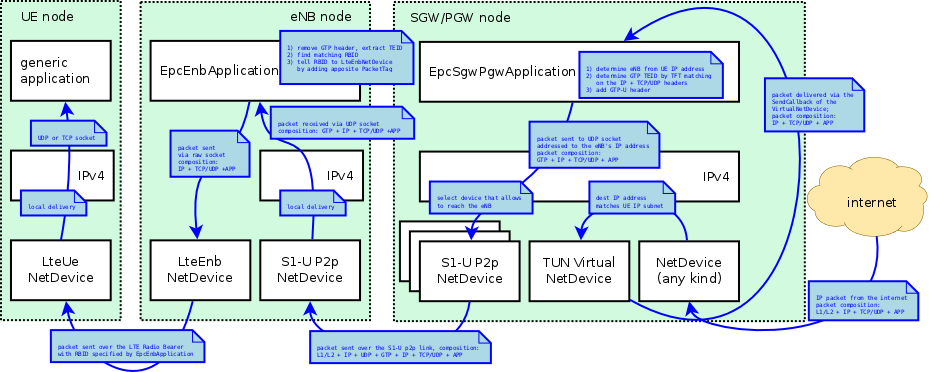
\includegraphics [width=0.95\textwidth] {DownloadUE.png}
  \caption{Поток данных нисходящей линии связи между интернетом и узлом UE \cite{LteSimDoc}}
  \label{img:DownloadUE}
\end{figure}

\begin{enumerate}
  \item Определяет eNB узел, к которому присоединен UE, смотря на IP-адрес назначения (который является адресом UE).
  \item Классифицирует пакеты, используя шаблоны транспортных потоков (TFT - Traffic Flow Templates), чтобы идентифицировать, какому ePS каналу он принадлежит. ePS каналы имеют карту соответсвия к S1-U каналам, так что эта операция возвращает идентификатор TEID (GTP-U Tunnel Endpoint Identifier), к которому принадлежит данный пакет.
  \item Добавляет соответствующие GTP-U-заголовки к пакету.
  \item Отправляет пакет через UDP-сокет к S1-U P2P NetDevice, адресуя к eNB, с которым соединен UE.
\end{enumerate}
Как следствие, пакес со сквозным IP заголовком с добавленными IP, UDP и GTP заголовками отправляется S1 соединение к eNB, где он принимается и доставляется локально (в качестве адреса назначения подставляется приватный адрес eNB). Локальный процесс доставки отправит пакет через UDP сокет к выделенному приложению EpcEnbApplication. Это приложение выполняет следующие операции:
\begin{enumerate}
  \item Удаляет заголовок GTP и извлекает TEID, который содержится в нем.
  \item Используя на взаимно-однозначное соответствие между S1-U каналами и радио каналами (который является 3GPP требованием), определяет идентификатор радиоканала (RBID -Radio Bearer ID), к которому принадлежит данный пакет.
  \item Записывает RBID в выделенном тег под названием LteRadioBearerTag, который добавляется к пакету.
  \item Пересылает пакет к приложению LteEnbNetDevice eNB узла через raw сокет.
\end{enumerate}
Следует отметить, что в этот момент, внешним заголовком пакета является сквозной IP заголовок, поскольку IP/UDP/GTP заголовки S1 стека протоколов уже были удалены. После приема пакета от EpcEnbApplication, LteEnbNetDevice будет извлекать RBID из LteRadioBearerTag, и на основе RBID определит экземпляр радиоканала (и соответствующие PDCP и RLC экземпляры протокола), которые затем используются для передачи пакета к UE через радиоинтерфейс LTE. В конце, приложение LteUeNetDevice узла UE получит пакет и доставит его локально через IP стек протоколов, которые в свою очередь доставит его к приложению на узле UE, которое является конечной точкой нисходящей линии связи.

В случае восходящего соединения, показанном на рис. \ref{img:UploadUE} , IP пакеты создаются приложением внутри UE, и передается локальным стеком протоколов TCP / IP к приложению LteUeNetDevice узла UE. LteUeNetDevice затем выполняет следующие операции:
\begin{enumerate}
  \item Классифицирует пакет, испоьзуя TFT, и определяет радиоканал, к которому принадлежит пакет (и соответствующие RBID).
  \item Определяет соответствующий экземпляр протокола PDCP, который является точкой входа LTE радио стеком протоколов для этого пакета.
  \item Посылает пакет к eNB через LTE радио стек протоколов.
\end{enumerate}
eNB принимает пакет через его сетевой интерфейс LteEnbNetDevice. Поскольку существует один экземпляр протокола PDCP и RLC для каждого радиоканала, LteEnbNetDevice способен определить RBID пакета. Это RBID затем записывается в LteRadioBearerTag, который добавляется к пакету. LteEnbNetDevice затем пересылает пакет EpcEnbApplication через сокет пакета.
При получении пакета EpcEnbApplication выполняет следующие операции:
\begin{enumerate}
  \item Извлекает RBID из тега LteRadioBearerTag в пакете.
  \item Определяет соответствующий EPS канал и GTP-U TEID за счет использования на взаимно-однозначное соответствие между S1-U каналами и радиоканалами.
  \item Добавляет GTP-U заголовок пакета, в том числе TEID, который был определен ранее.
  \item Посылает пакет на SGW/PGW узел через UDP сокет подключенный к S1-U сетевому точка-точка устройству.
\end{enumerate}

В этот момент пакет содержит S1-U IP, UDP и GTP заголовки в дополнение к первоначальному сквозному IP заголовку. Когда пакет поступает на соответствующий S1-U P2P NetDevice на узле SGW/PGW, он доставляется локально. Локальный процесс доставки направляет пакет к EpcSgwPgwApplication через соответствующий UDP сокет. EpcSgwPgwApplication затем удаляет заголовок GTP и пересылает пакет VirtualNetDevice. На данный момент, внешним заголовком пакета является сквозной IP заголовок. Следовательно, если адрес назначения в этот заголовке является удаленным узлом в интернете, пакет отправляется в интернет через соответствующие сетевое устройство NetDevice на узле SGW/PGW. В случае, если пакет адресован другому UE, IP стек SGW/PGW перенаправит пакет снова к сетевому устройству VirtualNetDevice, и пакет будет проходить через процесс доставки через нисходящее соединение для того, чтобы достичь пункта назначения UE.

\begin{figure} [h]
  \center
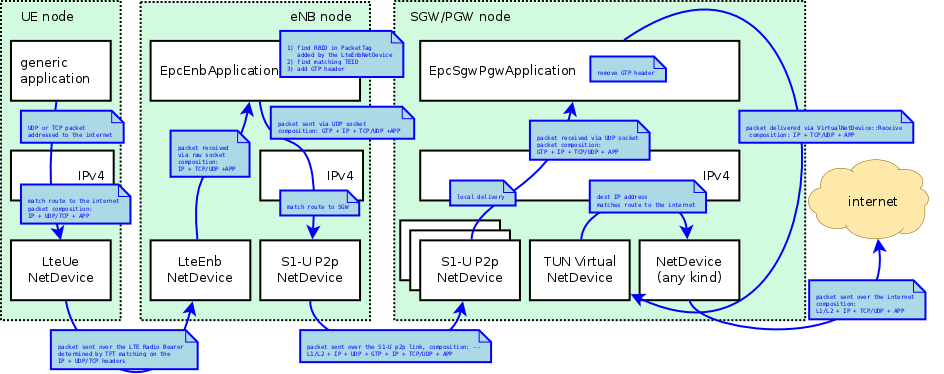
\includegraphics [width=0.95\textwidth] {UploadUE.png}
  \caption{Поток данных восходящей линии связи между узлом UE и интернетом \cite{LteSimDoc}}
  \label{img:UploadUE}
\end{figure}



\clearpage




